%%%%%%%%%%%%%%%%%%%%%%%%%%%%%%%%%%%%%%%%%%%%%%%%%%%%%%%%%%%%%%%%%%%%%%%%%%%%%%%%%%
\begin{frame}[fragile]\frametitle{}

\begin{center}
{\Large Machine/Deep Learning in spaCy}
\end{center}
\end{frame}

%%%%%%%%%%%%%%%%%%%%%%%%%%%%%%%%%%%%%%%%%%%%%%%%%%%%%%%%%%%%%%%%%%%%%%%%%%%%%%%%%%
\begin{frame}[fragile]\frametitle{Vectorization}

\begin{itemize}
\item Raw  text needs to be converted to numbers/vectors before using them in any Machine/Deep Learning algorithm.
\item One can generate word vectors or resue pre-trained word embedding models.
\item Similarity is one of the measures to assess quality of word embeddings, in terms of capturing semantics.
\end{itemize}
\end{frame}


%%%%%%%%%%%%%%%%%%%%%%%%%%%%%%%%%%%%%%%%%%%%%%%%%%%%%%%%%%%%%%%%%%%%%%%%%%%%%%%%%%
\begin{frame}[fragile]\frametitle{Vectorization in spaCy}

\begin{itemize}
\item spaCy’s small models (all packages that end in sm) don’t ship with word vectors, and only include context-sensitive tensors. 
\item Can still use the similarity() methods to compare documents, spans and tokens – but the result won’t be as good, 
\item individual tokens won’t have any vectors assigned. 
\item For real word vectors, you need to download a larger model
\end{itemize}
\end{frame}

%%%%%%%%%%%%%%%%%%%%%%%%%%%%%%%%%%%%%%%%%%%%%%%%%%%%%%%%%%%%%%%%%%%%%%%%%%%%%%%%%%
\begin{frame}[fragile]\frametitle{Example}

\begin{lstlisting}
import spacy

nlp = spacy.load("en_core_web_md")
tokens = nlp("dog cat banana afskfsd")

for token in tokens:
    print(token.text, token.has_vector, token.vector_norm, token.is_oov)
		
dog True 7.0336733 True
cat True 6.6808186 True
banana True 6.700014 True
afskfsd False 0.0 False
\end{lstlisting}

\begin{itemize}
\item Common words like cat and dog are so they’re part of the model’s vocabulary, and come with a vector, but not the ones like ``afskfsd''
\item ``lg'' model has 1 million unique vectors.
\end{itemize}
\end{frame}

%%%%%%%%%%%%%%%%%%%%%%%%%%%%%%%%%%%%%%%%%%%%%%%%%%%%%%%%%%%%%%%%%%%%%%%%%%%%%%%%%%
\begin{frame}[fragile]\frametitle{Similarity in spaCy}

\begin{itemize}
\item Can compare two objects, and make a prediction of how similar they are. 
\item Each Doc, Span and Token comes with a \lstinline|.similarity()|
\item Similarity is always subjective – whether “dog” and “cat” are similar in general vector model sense.
\item Similarity is determined using word vectors
\item Multi-dimensional meaning representations of words
\item Generated using an algorithm like Word2Vec and lots of text
\item Can be added to spaCy's statistical models
\item Default: cosine similarity, but can be adjusted
\item Doc and Span vectors default to average of token vectors
\item Short phrases are better than long documents with many irrelevant words
\end{itemize}
\end{frame}
%%%%%%%%%%%%%%%%%%%%%%%%%%%%%%%%%%%%%%%%%%%%%%%%%%%%%%%%%%%%%%%%%%%%%%%%%%%%%%%%%%
\begin{frame}[fragile]\frametitle{Example}

\begin{lstlisting}
import spacy

nlp = spacy.load("en_core_web_md")  # make sure to use larger model!
tokens = nlp("dog cat banana")

for token1 in tokens:
    for token2 in tokens:
        print(token1.text, token2.text, token1.similarity(token2))
		
dog dog 1.0
dog cat 0.80168545
dog banana 0.24327643
cat dog 0.80168545
cat cat 1.0
cat banana 0.28154364
banana dog 0.24327643
banana cat 0.28154364
banana banana 1.0
\end{lstlisting}

\begin{itemize}
\item Common words like cat and dog are so they’re part of the model’s vocabulary, and come with a vector, but not the ones like ``afskfsd''
\item ``lg'' model has 1 million unique vectors.
\end{itemize}
\end{frame}

%%%%%%%%%%%%%%%%%%%%%%%%%%%%%%%%%%%%%%%%%%%%%%%%%%%%%%%%%%%%%%%%%%%%%%%%%%%%%%%%%%
\begin{frame}[fragile]\frametitle{Exercise}

\begin{itemize}
\item Load the medium "en_core_web_md" model with word vectors.
\item Print the vector for "bananas" using the token.vector attribute.
\item Use the doc.similarity method to compare doc1 to doc2 and print the result.

\end{itemize}


\begin{lstlisting}
import spacy

# Load the en_core_web_md model
nlp = ____

# Process a text
doc = nlp("Two bananas in pyjamas")

# Get the vector for the token "bananas"
bananas_vector = ____.____
print(bananas_vector)

doc1 = nlp("It's a warm summer day")
doc2 = nlp("It's sunny outside")

# Get the similarity of doc1 and doc2
similarity = ____.____(____)
print(similarity)
\end{lstlisting}


\end{frame}


%%%%%%%%%%%%%%%%%%%%%%%%%%%%%%%%%%%%%%%%%%%%%%%%%%%%%%%%%%%%%%%%%%%%%%%%%%%%%%%%%%
\begin{frame}[fragile]\frametitle{Customizing word vectors}

\begin{itemize}
\item Custom word vectors can be trained using a number of open-source libraries, such as Gensim.
\item For everyday use, we want to convert the vectors model into a binary format that loads faster and takes up less space on disk.
This will output a spaCy model in the directory /tmp/la\_vectors\_wiki\_lg
\end{itemize}

\begin{lstlisting}
wget https://s3-us-west-1.amazonaws.com/fasttext-vectors/word-vectors-v2/cc.la.300.vec.gz
python -m spacy init-model en /tmp/la_vectors_wiki_lg --vectors-loc cc.la.300.vec.gz

nlp_latin = spacy.load("/tmp/la_vectors_wiki_lg")
doc1 = nlp_latin("Caecilius est in horto")
doc2 = nlp_latin("servus est in atrio")
doc1.similarity(doc2)
\end{lstlisting}


\end{frame}

%%%%%%%%%%%%%%%%%%%%%%%%%%%%%%%%%%%%%%%%%%%%%%%%%%%%%%%%%%%%%%%%%%%%%%%%%%%%%%%%%%
\begin{frame}[fragile]\frametitle{ML inside spaCy}

\begin{itemize}
\item spaCy’s models are statistical and every “decision” they make – for example, which part-of-speech tag to assign, or whether a word is a named entity – is a prediction. 
\item Usual ML training, testing, evaluation process is followed.
\end{itemize}

\begin{center}
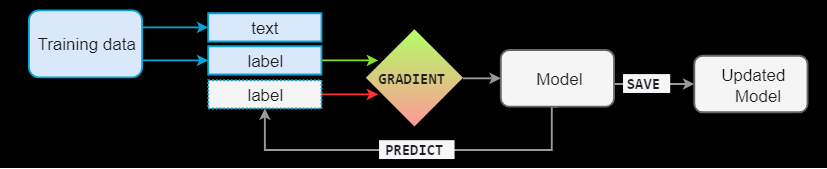
\includegraphics[width=0.6\linewidth,keepaspectratio]{spacy16}
\end{center}


\end{frame}